\section{Analisi cinetostatica}
Una volta effettuata la cinematica e dinamica del sistema in questo capitolo presentiamo l'analisi cinetostatica. In particolare andremo a concentrarci sui punti di singolarità, sul numero di condizionamento e per concludere analizzeremo lo spazio di lavoro del manipolatore.
\begin{figure}[ht]
	\begin{center}
		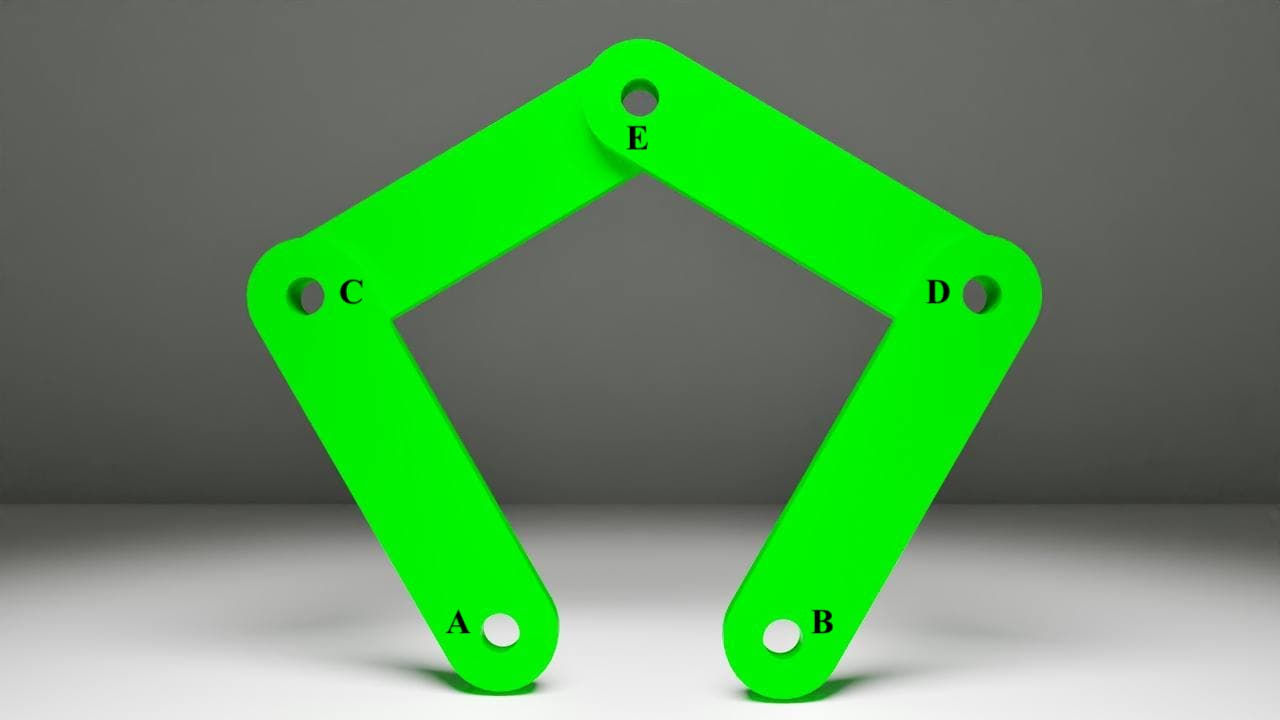
\includegraphics[scale=0.3]{Immagini/Singolarity/0}
		\caption{Posizione standard manipolatore}
	\end{center}
\end{figure}
\subsection{Punti di singolarità}
Nell'ambito matematico, una singolarità è un punto nel quale un oggetto non è definito, oppure un punto nel quale l'oggetto non ha un comportamento normale, nel nostro caso i punti di singolarità sono punti che vanno a delimitare lo spazio di lavoro del robot. Definiamo \textit{workspace} del manipolatore una parte del piano [x,y] nel quale il robot ha un funzionamento normale e non presenta problematiche\footnote{Nel caso in cui il manipolatore dovesse passare per un punto di singolarità potrebbero verificarsi problematiche sia nel seguire la traiettoria che a livello meccanico, arrivando nel peggiore dei casi alla rottura.}. Considerando l'immagine \ref{fig:PKM} si possono identificare cinque casi di singolarità. Di conseguenza il robot avrà come spazio di lavoro, tutto lo spazio che è interno (delimitato) da queste configurazioni.
\subsubsection*{Primo e secondo caso}
\addcontentsline{toc}{subsubsection}{Primo e secondo caso}
In questo primo caso abbiamo $\overrightarrow{CD}$ che è parallelo a $\overrightarrow{DE}$, schematicamente possiamo andarlo a rappresentare nel seguente modo
\begin{figure}[ht]
	\begin{center}
		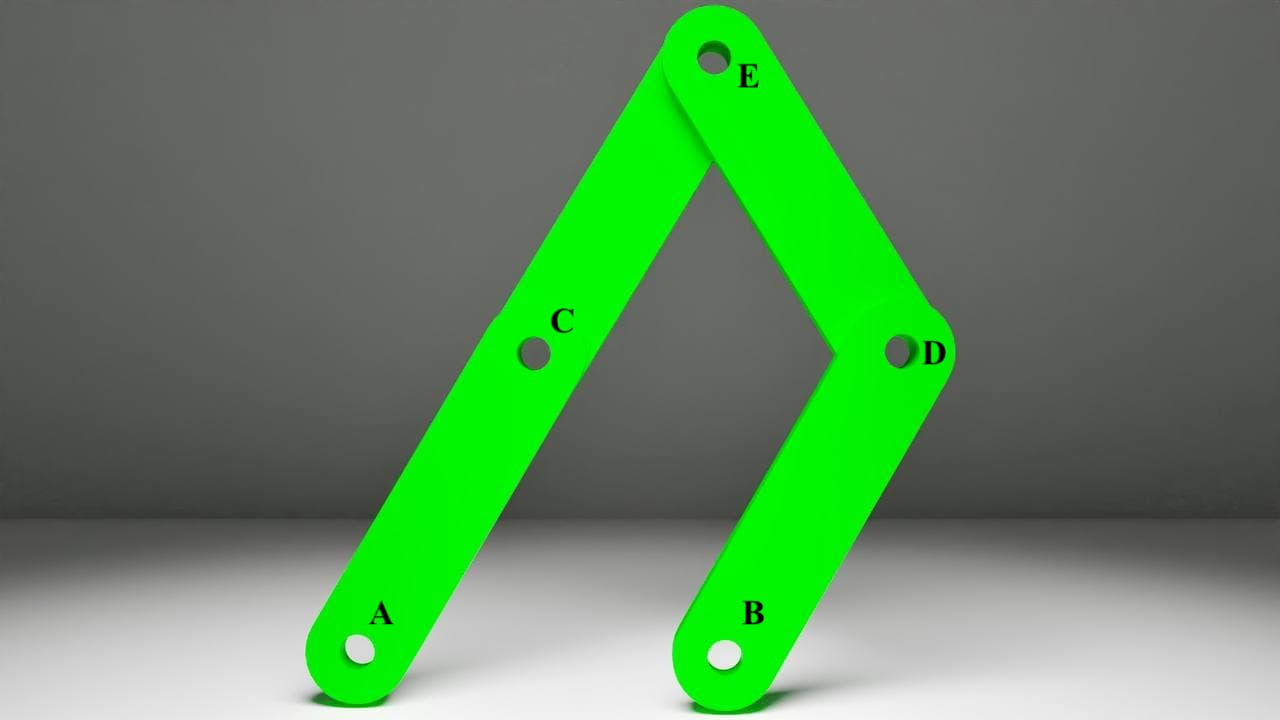
\includegraphics[scale=0.3]{Immagini/Singolarity/1}
		\caption{Caso 1 singolarità}
	\end{center}
\end{figure}
\\Analiticamente: $||\overrightarrow{AC}||^2 = (l+l)^2$ quindi: 
\begin{equation*}
	\Bigg| \begin{bmatrix}
		-d  \\ 0
	\end{bmatrix} - \begin{bmatrix}
	x \\ y
\end{bmatrix}\bigg|^2 = 4l^2
\end{equation*}
\begin{equation*}
\bigg|	\begin{bmatrix}
		-d-x \\ -y
	\end{bmatrix}\Bigg|^2 = 4l^2
\end{equation*}
Svolgendo il modulo troviamo 
\begin{equation*}
	d^2 + 2dx + x^2 +y^2 = 4l^2
\end{equation*}
Facendo variare x ricaviamo la y come:
\begin{equation}
    y_1 = \sqrt{4l^2-(x-d)^2}
\end{equation}
Per quanto riguarda il secondo caso è simmetrico al primo, abbiamo la catena $\overrightarrow{AB}$ parallela a $\overrightarrow{BC}$:
\begin{figure}[ht]
	\begin{center}
		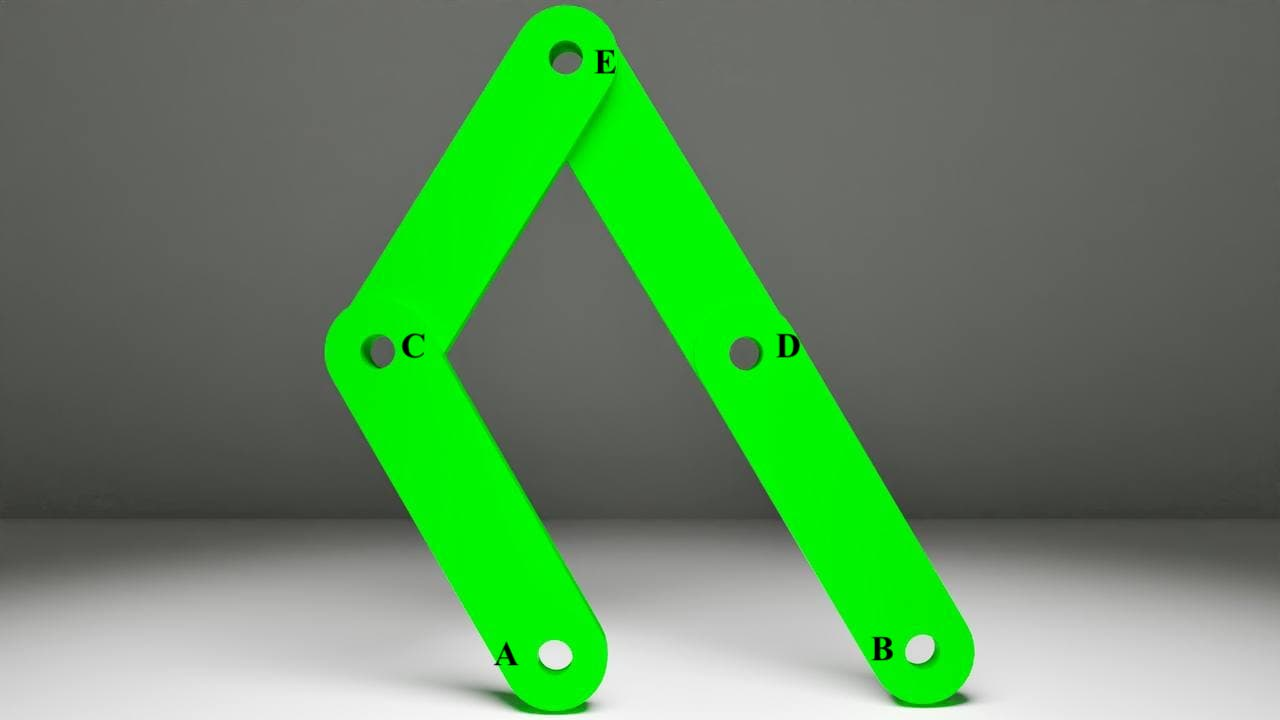
\includegraphics[scale=0.3]{Immagini/Singolarity/2}
		\caption{Caso 2 singolarità}
	\end{center}
\end{figure}
\\Il procedimento è simile a prima, lasciando sempre la x libera possiamo trovare la y come:
\begin{equation}
    y_2 = \sqrt{4l^2-(x+d)^2}
\end{equation}
Entrambi i casi producono come risultato una circonferenza.
\subsubsection*{Terzo caso}
\addcontentsline{toc}{subsubsection}{Terzo caso}
Il terzo caso di singolarità avviene quando i due link non motorizzati sono paralleli, abbiamo tre giunti allineati tra di loro rendendo la configurazione labile. Per poter uscire da questa singolarità abbiamo la necessità di una maggior coppia.
\begin{figure}[ht]
	\begin{center}
		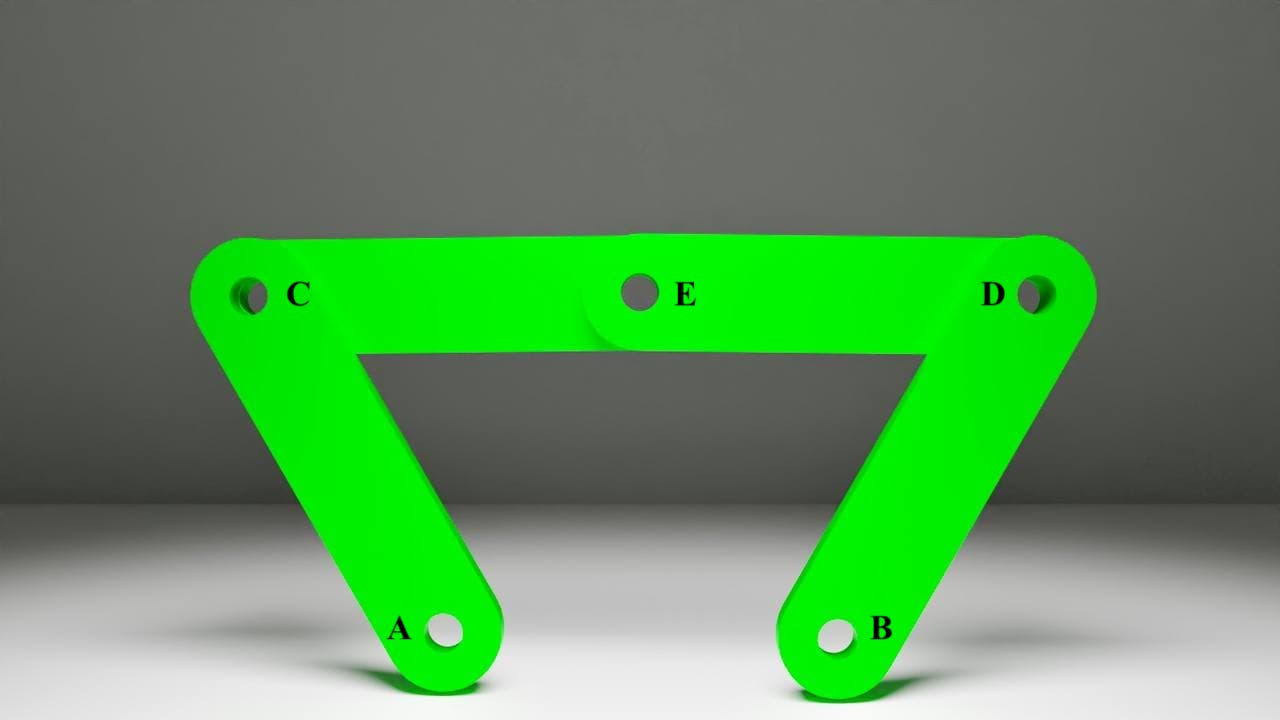
\includegraphics[scale=0.3]{Immagini/Singolarity/5}
		\caption{Caso 3 singolarità}
	\end{center}
\end{figure}
\\Per quanto riguarda la soluzione, andiamo inizialmente a trovare la posizione del punto D $[x_D,y_D]$: facciamo l'intersezione tra due circonferenze la prima ha centro in E con raggio l, la seconda ha centro in B con raggio 2l; possiamo esprimere le equazioni come:
\begin{equation}
	\begin{cases}
		(x_D-d)^2 +y_D^2= l \\
		(x_D-l\cos\theta_1+d)^2 + (y_D-l\sin\theta_1)^2 = 4l^2
	\end{cases}
\end{equation}
Svolgendo i quadrati:
\begin{equation*}
	\begin{cases}
	 x_D^2-2dx_D+d^2+y_D^2 = l^2 \\
	 x_D^2+ l^2 + d^2-2ld\cos\theta_1 -2x_Dl\cos\theta_1+2x_Dd + y_D^2-2y_Dl\sin\theta_1 = 4l^2-l^2
	\end{cases}
\end{equation*}
Sottraendo la prima equazione nella seconda otteniamo: 
\begin{equation*}
	x_D(-l\cos\theta_1+2d) -y_Dl\sin\theta_1 - ld\cos\theta_1 = l^2
\end{equation*}
Otteniamo x in funzione di y come:
\begin{equation*}
	x_{D} = \frac{l^2+y_{D}l\sin\theta_1+ld\cos\theta_1}{2d-l\cos\theta_1}
\end{equation*}
 Sostituendo la x nella prima equazione possiamo ottenere y in funzione di $\theta_1$:
 \begin{equation}
 	y_{D} = \frac{-b\pm \sqrt{b^2-4ac}}{2a}
 \end{equation}
 dove:
\begin{equation*}
	a = l^2\sin^2\theta_1 + 4d^2-4dl\cos\theta_1 + l^2\cos^2\theta_1
\end{equation*}
\begin{equation*}
	b = 2l^3\sin\theta_1 + 2dl^2\sin\theta_1\cos\theta_1-2dl\sin\theta_1(2d-2l\cos\theta_1)
\end{equation*}
\begin{equation*}
	c = l^2(l^2+d^2\cos^2\theta_1+2ld\cos\theta_1)-2dl(l+d\cos\theta_1)(2d-l\cos\theta_1)+(d^2-l^2)(2d-l\cos\theta_1)^2
\end{equation*}
Facendo variare $\theta_1$ troviamo $x_D$ e $y_D$. Per poter trovare la posizione dell'\textit{end-effector} facciamo la media tra la posizione del punto D e del punto B.
\begin{equation}
	x_3 = \frac{x_D-d+l\cos\theta_1}{2}, y_3 = \frac{y_B+l\sin\theta_1}{2}
\end{equation}
\subsubsection*{Quarto e quinto caso}
\addcontentsline{toc}{subsubsection}{Terzo e quarto caso}
Il quarto e quinto sono casi di singolarità non realizzabili nella pratica, ma sono di interesse teorico. Il primo prevede che la posizione dell'end-effector coincida con la posizione del primo giunto motorizzato mentre nell'altro che coincida con il secondo giunto motorizzato. Come soluzioni avremo semplicemente due punti e possiamo andare a calcolarli nei seguenti modi:
\begin{figure}[!ht]
	\begin{subfigure}{.5\textwidth}
		\centering
		% include first image
		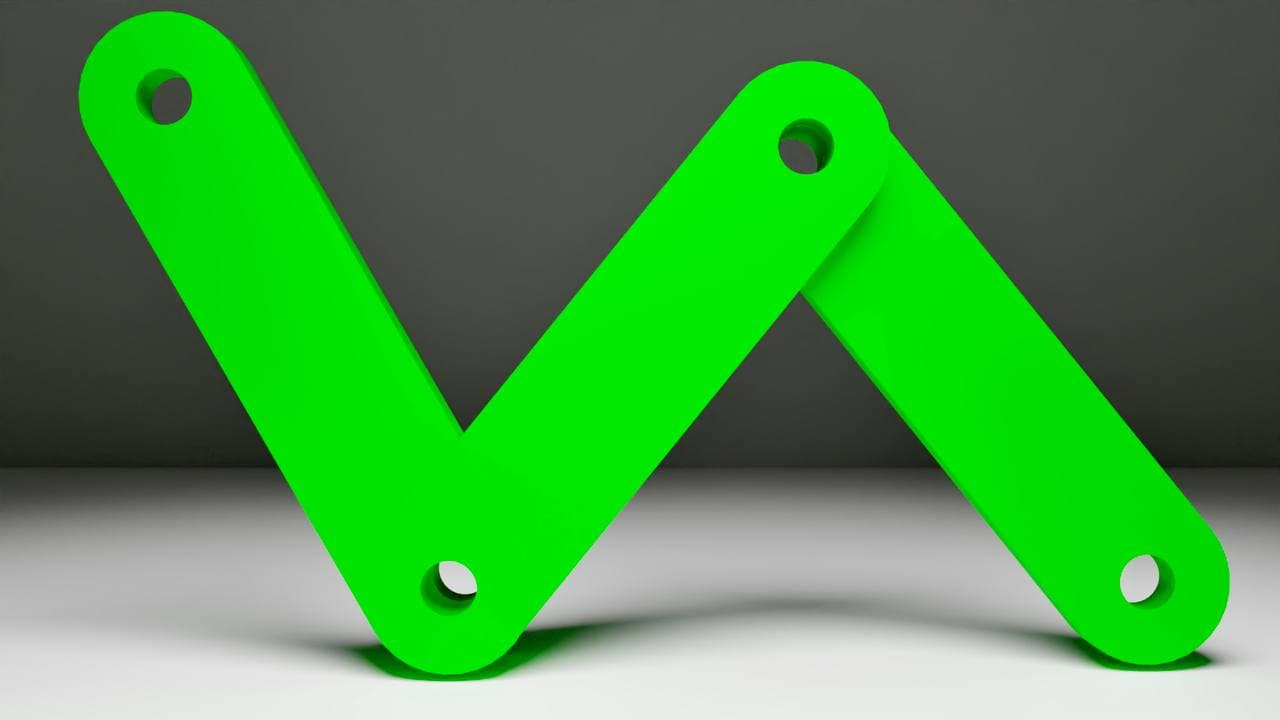
\includegraphics[width=.9\linewidth]{Immagini/Singolarity/3}
		\label{fig:sing4}
	\end{subfigure}
	\begin{subfigure}{.5\textwidth}
		\centering
		% include second image
		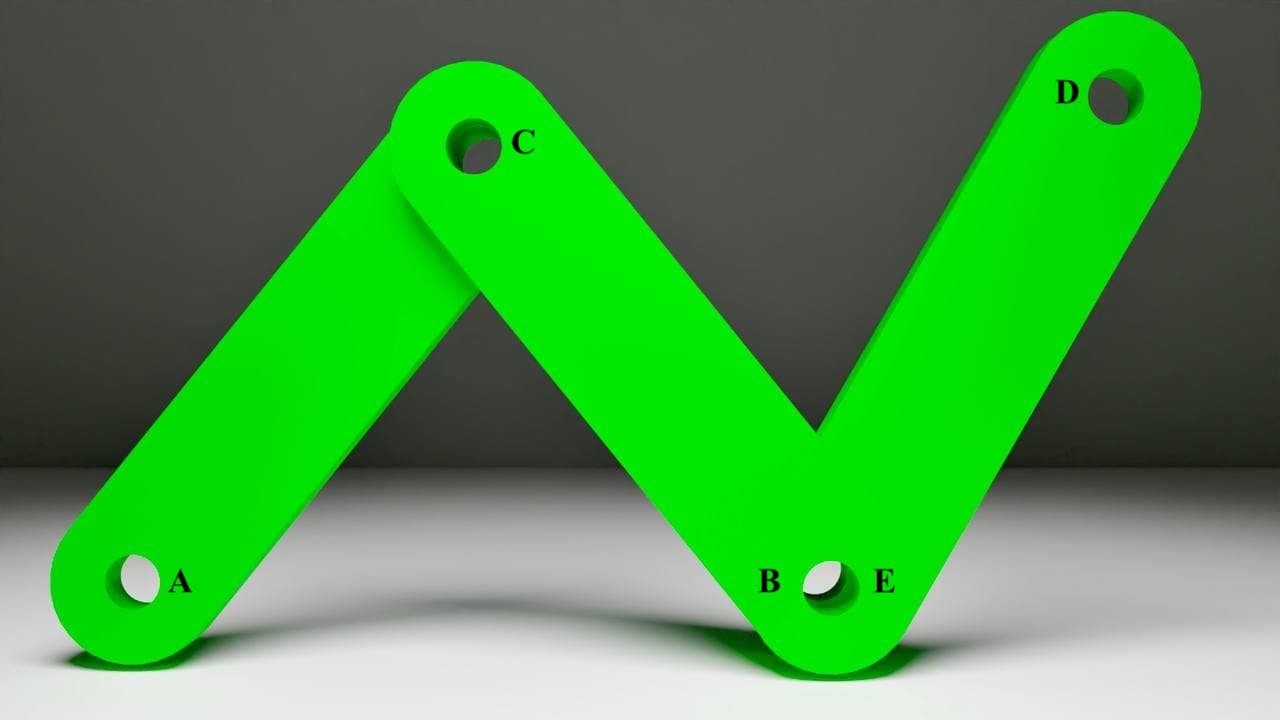
\includegraphics[width=.9\linewidth]{Immagini/Singolarity/4}  
		\label{fig:sing5}
	\end{subfigure}
	\caption{Caso 4 e 5 singolarità}
	\label{Caso4Sing}
\end{figure}
\\Possiamo trovare le soluzione del quarto caso imponendo \begin{equation}|\overrightarrow{EC}| = 0 \rightarrow x=d, y = 0
\end{equation}
e per il quinto caso 
\begin{equation}
	|\overrightarrow{AC}| = 0 \rightarrow x=-d, y=0
\end{equation}
Per delimitare i confini di operabilità del manipolatore sono stati uniti tutti e cinque i casi di singolarità. Nella figura seguente è fornita una rappresentazione sul piano cartesiano dell'unione di questi luoghi di singolarità, facciamo notare che non tutti i punti sono fisicamente raggiungibili dal robot per come è stato progettato; in particolare la posizione y dell'\textit{end-effector} non potrà mai essere negativa.
\begin{figure}[ht]
\begin{center}
    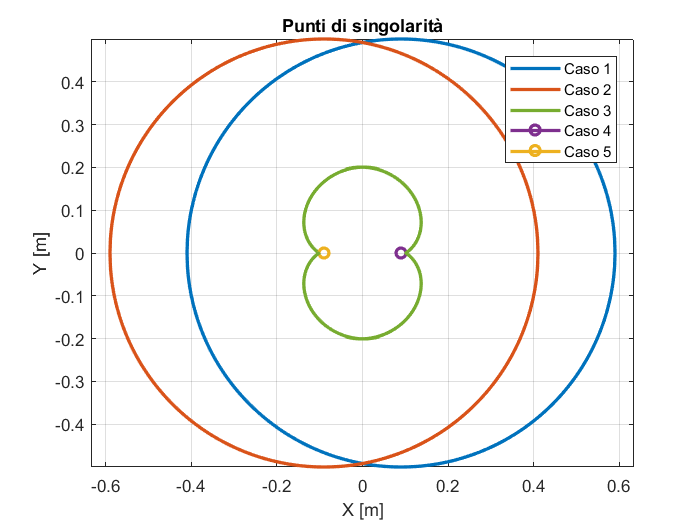
\includegraphics[scale=0.6]{Immagini/Singolarity/SingNewNew}
    \caption{Punti di singolarità}
    \label{puntiSing}
\end{center}
\end{figure}
\subsection{Manipolabilità}
La manipolabilità ci permette di avere una rappresentazione geometrica delle capacità che ha un punto del nostro sistema. Per andare a calcolarla abbiamo bisogno dell'equazione \ref{eq:J12}, vista nella sezione \ref{sec:CalcoloVelCin}.
\\Andiamo a definire la matrice
\begin{equation}
    J_{man} = JJ^T
\end{equation}
Da questa possiamo ricavare gli autovalori $\lambda_1, \lambda_2$. Definiamo  l'indice di manipolabilità \textbf{r} come:
\begin{equation}
    r = \frac{\max(\lambda_1,\lambda_2)}{\min(\lambda_1,\lambda_2)}
\end{equation}
Questo numero può variare tra 1 e $+\infty$, più è piccolo e meno si rischia di andare in singolarità. Lo spazio analizzato ha come estremi:
\begin{equation*}
	\begin{split}
		-0.3 \le x \le 0.3 \\
		0.1 \le y \le 0.5
	\end{split}
\end{equation*} 
Rappresentiamo il numero di condizionamento tramite i seguenti grafici: 
\begin{figure}[!ht]
	\begin{subfigure}{.55\textwidth}
		\centering
		% include first image
		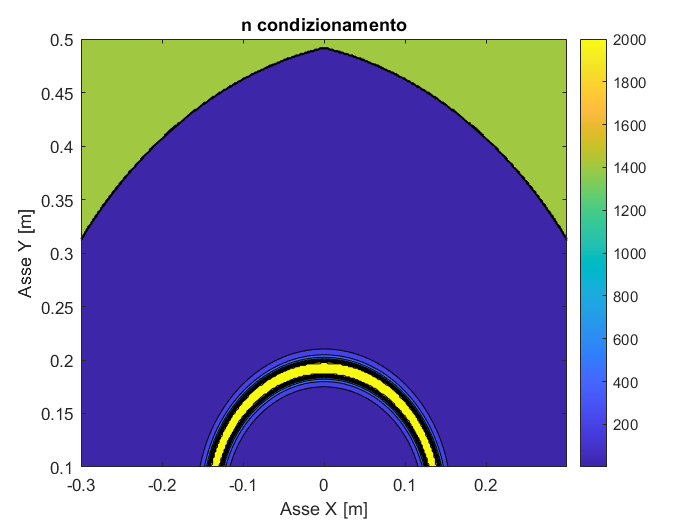
\includegraphics[width=.9\linewidth]{Immagini/Singolarity/Ncond}
		\label{fig:ncond}
	\end{subfigure}
	\begin{subfigure}{.55\textwidth}
		\centering
		% include second image
		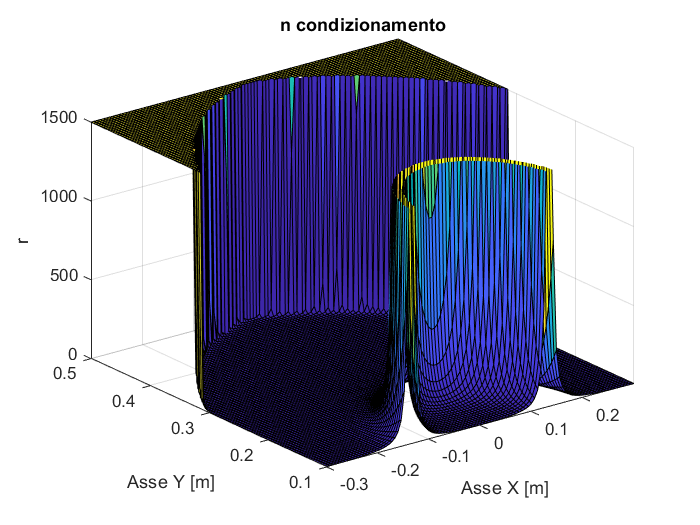
\includegraphics[width=.9\linewidth]{Immagini/Singolarity/Ncond_surf}  
		\label{fig:nconds}
	\end{subfigure}
	\caption{Numero di condizionamento}
	\label{NumCondiz}
\end{figure}
\\Nel primo grafico viene mostrato il piano x,y ed il numero di condizionamento è definito come una colormap, i punti di color blu sono quelli con un r piccolo ed in questi non siamo in condizioni di singolarità, invece quelli tendenti al verde/giallo sono i casi di singolarità che abbiamo visto prima. Nella seconda figura possiamo vedere la stessa rappresentazione però in tre dimensioni, utilizziamo l'asse z per rappresentare il numero di condizionamento; anche qua le zone di singolarità sono chiaramente visibili.

\subsection{Workspace}
Dalle analisi appena effettuate sui punti di singolarità e sul numero di condizionamento è stato possibile descrivere i limiti di lavoro del manipolatore. In prima battuta ci si è concentrato sull'analizzare gli angoli di movimentazione dei giunti e i loro vincoli, in particolare il link sinistro con angolo $\theta_1$ può effettuare un movimento da $60^\circ$ fino a $210^\circ$, mentre il link destro da $-30^\circ$ e $150^\circ$. Questa limitata mobilità è data dai vincoli che ci sono tra le due braccia, infatti, se a livello teorico si possono ottenere configurazioni particolari come quella vista in figura \ref{Caso4Sing} nella pratica non è possibile muovere né manualmente né automaticamente i giunti per ottenere quei casi, l'unico modo possibile è quello di smontare e rimontare il manipolatore al contrario. \\Possiamo andare a rappresentare gli angoli di movimentazione mediante la seguente immagine: 
\begin{figure}[ht]
	\begin{center}
		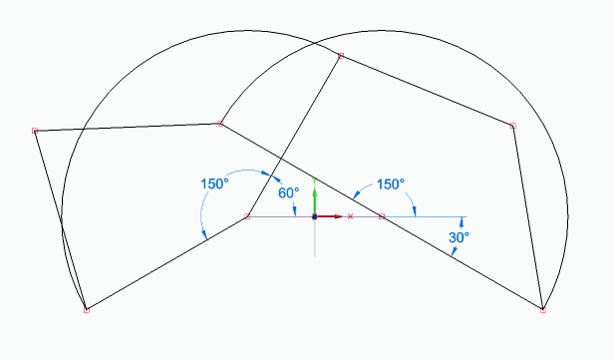
\includegraphics[scale=0.56]{Immagini/Singolarity/workangle}
		\caption{Angoli di movimentazione dei giunti motorizzati}
	\end{center}
\end{figure}
\\A partire dai limiti di lavoro è stato identificato uno spazio buono dove il manipolatore può operare non raggiungendo i punti singolari. Questo luogo è stato descritto mediante un rettangolo:
\begin{figure}[ht]
	\begin{center}
		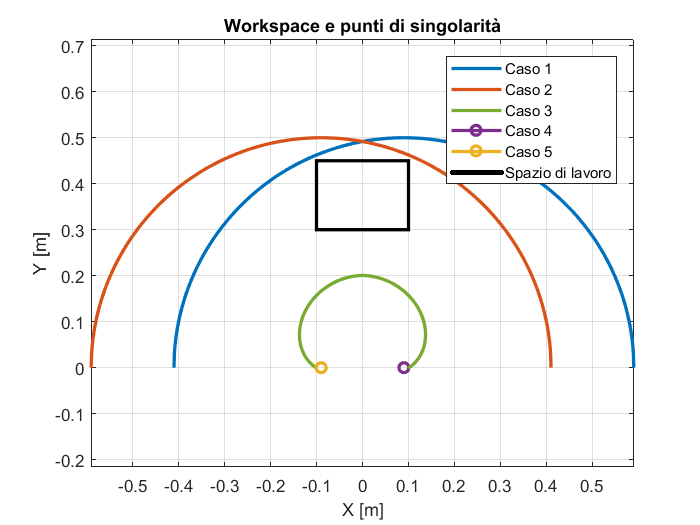
\includegraphics[scale=0.55]{Immagini/Singolarity/WorksingNew}
		\caption{\textit{Workspace} 5R}
	\end{center}
\end{figure}
\\Con estremi:
\begin{equation*}
	\begin{split}
		-0.1 \le x \le 0.1 \\
		0.3 \le y \le 0.45
	\end{split}
\end{equation*}
\\Successivamente, per verificare che lo spazio di lavoro fosse corretto e rispettasse tutte le condizioni è stata fatta un'analisi sul numero di condizionamento del \textit{workspace}:
\begin{figure}[ht]
	\begin{center}
		\includegraphics[scale=0.55]{Immagini/Singolarity/ncondsl}
		\caption{Numero di condizionamento workspace}
	\end{center}
\end{figure}
\\Su tutto il piano x,y si nota come il numero di condizionamento assume valori bassi, questo implica che non vi è singolarità, gli unici punti critici sono quelli esterni, nei quali il valore è vicino a 6, (comunque minore di $\infty$), questi punti vanno a rappresentare casi nei quali il manipolatore avrà più difficoltà a muoversi, ma non sono veri e propri punti di singolarità.